\documentclass{beamer} 
\usepackage{ragged2e}
\usepackage{etoolbox}
\usepackage{lipsum}

\apptocmd{\frame}{}{\justifying}{} % Allow optional arguments after frame

\title{Robotic Platform for enabling students to learn robotics} 


\usetheme{PaloAlto}
\begin{document}  
\maketitle

\begin{frame}
\frametitle{Roadmap}
\begin{itemize}
\item Introduction\textbackslash Motivation
\item Market Research\textbackslash Literature Survey
\item Hardware Requirements
\item Software Requirements
\item Implementation
\item Feasibility
\item References
\end{itemize}
\end{frame}
  
\section{One}  
\begin{frame}
\frametitle{Introduction\textbackslash Motivation}
\begin{center}
\justifying
While there has been tremendous progress in schools adopting robotics as compared to a decade ago, the subjects of robotics and programming are still niche subjects and not easily accessible to all. The existing systems which aim to encourage students to explore the world of robotics and automation are too expensive and out of reach of most students. Furthermore, they are not easy to use and require sufficient knowledge to operate them.

There is a need in the market for a low cost all-in-one solution that can help young students to learn and practice robotics and programming to build solutions and implement ideas which, till now, were only not easily implementable by them. The proposed system will therefore enable these young minds to create and build applications using features like GUI based event driven programming as well as native python programming. The system will enable the users to build various applications like automation, robotic companions, robotic assistants, etc.
\end{center}
\end{frame}  

\section{Two}  
\begin{frame}
\frametitle{Market Research\textbackslash Literature Survey}
\begin{center}
\justifying
\begin{itemize}
\item Lego Mindstorms
\begin{itemize}
\item Lego Mindstorms is a kit which can be programmed to do a particular task. To
program the Lego Mindstorms kit, the users need to use the Lego Mindstorms
software.
\item Cost - Onwards of 1 lakh rupees.
\item Advantage
	\begin{itemize}
	\item Lego Mindstorms uses drag-and-drop GUI based programming.
	\end{itemize}
\item Disadvantage
	\begin{itemize}
	\item The kits are very costly and the kits do not come bundled with all the sensors.
	\end{itemize}	
\end{itemize}
\end{itemize}
\end{center}
\end{frame}  

\begin{frame}
\frametitle{Market Research\textbackslash Literature Survey}
\begin{center}
\justifying
\begin{itemize}
\item Nao Humanoid
\begin{itemize}
\item Nao is a humanoid robot which can be programmed using its own IDE to perform any task.
\item The Nao is used in various industries and serves multiple purposes.
\item The cost of the Nao humanoid for educational purposes is Rs. 17 lakhs and thus it puts it out of the reach of almost all students and universities.
\end{itemize}

\end{itemize}
\end{center}
\end{frame}  

\begin{frame}
\frametitle{Market Research\textbackslash Literature Survey}
\begin{center}
\justifying
\begin{itemize}
\item Basic IoT Kits
\begin{itemize}
\item Colleges currently use barebones IoT learning kits which come with a few sensors, controllers and wires.Though they are great to learn IoT and robotics, they are not useful in building applications.
\item Furthermore, complex programming and electronics knowledge is required to operate them and therefore young school going students cannot use them.
\item There is a dire need in the market for a low cost solution which features all the advantages of the current products but one which is low cost and accessible to all.
\end{itemize}
\end{itemize}
\end{center}
\end{frame}

\section{Three}  
\begin{frame}
\frametitle{Hardware Requirements}
\begin{center}
\justifying
\begin{itemize}
\item Raspberry Pi
\item Motors
\item Battery
\item Jumper Cables
\item Sensors
	\begin{itemize}
	\item Gyroscope
	\item Ultrasonic
	\item IR
	\item Photo-diode
	\item Temperature sensor
	\item Camera Module 
	\end{itemize}	
\end{itemize}
\end{center}
\end{frame}  

\section{Four}  
\begin{frame}
\frametitle{Software Requirements}
\begin{center}
\justifying
\begin{itemize}
\item Blockly - block programming language (Open-Source) or MIT Scratch programming language (Based on Blockly).
\item Anaconda Python distribution (Open-Source).
\item SSH and VNC server/client (Open-Source).
\end{itemize}
\end{center}
\end{frame}  

\section{Five}  
\begin{frame}
\frametitle{Implementation}
\begin{center}
\justifying
\begin{itemize}
\item The users will be able to control the robot using two methods. New and inexperienced programmers will be able to program the robot using the GUI driven programming language which will be bundled with the system. Experienced programmers who need more flexibility have the option of using traditional programming languages like Python to control the robot. The core of the system will be a Raspberry Pi micro-controller board which has user programmable GPIO ports.

\item Both the methods of controlling the robot are directly tied to the user programmable GPIO ports and thus both the methods of programming will be equally effective at enabling the users to make their applications.
\end{itemize}
\end{center}
\end{frame}  

\begin{frame}
\frametitle{Implementation}
\begin{center}
\justifying
\begin{itemize}
\item The Raspberry Pi runs on a Linux based operating system. A monitor, keyboard and mouse are required to operate the Raspberry Pi. But we intend to make it simpler for the end user. Instead of attaching peripherals to the board, we plan to use the Secure Shell Protocol (SSH) along with VNC so that the users can seamlessly connect to the board and access all of its features from their own laptop/ computer. Thus, the Raspberry Pi acts as another peripheral to the user’s computer.

\item The GUI based programming can be done using blocks. Open source software like Blockly (developed by Google) and MIT Scratch(based on Blockly) can be used here to make an interactive IDE in which the user arranges the required blocks to form a flowchart. The Blockly framework will then convert this arrangement of blocks into meaningful code which can be run natively by the Raspberry Pi. 
\end{itemize}
\end{center}
\end{frame}   

\begin{frame}
\frametitle{Implementation}
\begin{center}
\justifying
\begin{itemize}
\item This is especially useful in schools where the students are not well versed with coding but are able to think in terms of flowcharts and processes to form a Blockly program which can then be used to control the robot. No programming experience is needed to make such programs. Only ideas about the applications and designing of flowcharts are expected make programs.

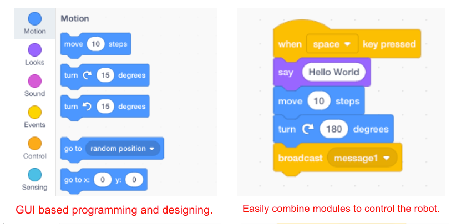
\includegraphics[height=.5\textheight]{Images/one.png}

\end{itemize}
\end{center}
\end{frame} 

\begin{frame}
\frametitle{Implementation}
\begin{center}
\justifying

\begin{itemize}
\item On the other hand for experienced developers who need more flexibility in their applications,
a Python library will be available to import into their code so that they can over look the basic
functionalities of the robot like locomotion, sensor interfacing, etc. and focus on the essential
ideas of their applications. This will enable them to make their applications quickly and
easily.

\end{itemize}
\end{center}
\end{frame} 

\begin{frame}
\frametitle{Implementation}
\begin{center}
\justifying
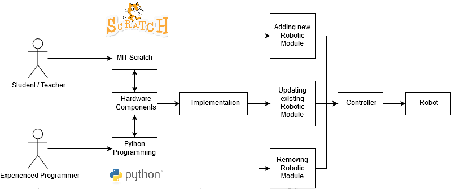
\includegraphics[height=.5\textheight]{Images/two.png}
\end{center}
\end{frame} 

\section{Six}
\begin{frame}
\frametitle{Feasibility}
\begin{center}
\justifying
\begin{itemize}
\item Operational Feasibility
	\begin{itemize}
	\item The intended system is easier to use and has more development features as com-pared to other solutions that are already available in the market.	
	\item The intended system can be programmed to be suitable for applications in various industries and organisations.
	\item The platform is customisable and will cater to both new as well as experienced
programmers.
	\item The platform covers the advantages of Lego Mindstorms and Nao humanoid and overcomes most of their drawbacks as well.
	\end{itemize}
\end{itemize}
\end{center}
\end{frame} 

\begin{frame}
\frametitle{Feasibility}
\begin{center}
\justifying
\begin{itemize}
\item Technical Feasibility
\begin{itemize}
\item Most of the components used are open source and freely available to reuse.
\item The hardware components meet the requirements of the system and are inexpensive and easily obtainable.
\item The intended system will be able to run efficiently on single board computers like the Raspberry Pi.
\end{itemize}
\end{itemize}
\end{center}
\end{frame} 

\begin{frame}
\frametitle{Feasibility}
\begin{center}
\justifying
\begin{itemize}
\item Economic Feasibility
\begin{itemize}
\item The financial resources to build this project are small and within the budget.
\item There is a need in the market for such a product and therefore there will be a demand for this product which in turn will generate a considerable revenue.
\item It is cost effective and accessible to all.
\end{itemize}
\end{itemize}
\end{center}
\end{frame} 

\section{Seven}
\begin{frame}
\frametitle{References}
\begin{center}
\justifying
\begin{itemize}
\item Roberto de Souza Baptista ; Marina Moreira ; Rafael Lima ; Mariana Bernardes - “Project Edubot : Teaching Robotics to High School Students”. Published in: 2018 Latin American Robotic Symposium, 2018 Brazilian Symposium on Robotics (SBR) and 2018 Workshop on Robotics in Education (WRE).
\item Ryan Connaughton ; Matthew Modlin - “A modular and extendable robotics platform for education”. Published in: 2009 39th IEEE Frontiers in Education Conference.
\item Yinong Chen ; Zhizheng Zhou - “Robots as a service in Computing Curriculum”. Published in: 2015 IEEE Twelfth International Symposium on Autonomous De- centralized Systems.
\end{itemize}
\end{center}
\end{frame} 

\begin{frame}
\frametitle{References}
\begin{center}
\justifying
\begin{itemize}
\item Blockly programming language - (https://developers.google.com/blockly).
\item MIT Scratch language - (https://scratch.mit.edu).
\item Sustainable Development Goals for Quality Education 
(https://www.undp.org/content/undp/en/home/
\\ sustainabledevelopmentgoals
\\ /goal4qualityeducation.htmltargets).
\end{itemize}
\end{center}
\end{frame} 

\end{document}